%--------------------------------------
%ELECTROTECHNIQUE - SCHEMA DE LIAISON A LA TERRE
%--------------------------------------

%utiliser les environnement \begin{comment} \end{comment} pour mettre en commentaire le préambule une fois la programmation appelée dans le document maître (!ne pas oublier de mettre en commentaire \end{document}!)

\begin{comment}

\documentclass[a4paper, 11pt, twoside, fleqn]{memoir}

\usepackage{AOCDTF}

\marqueurchapitre
\decoupagechapitre{1} %juste pour éviter les erreurs lors de la compilation des sous-programmations (passera en commentaire)

%lien de l'éditeur : https://www.mathcha.io/editor/1l8zXhV1HvqhK5rxB1Tm71NwrCP9yd7yHp7MQ6o

%--------------------------------------
%corps du document
%--------------------------------------

\begin{document} %corps du document
	\openleft %début de chapitre à gauche

\end{comment}

\begin{figure}[h]
\caption{Boucle de défaut du courant $I_d$ sur L1}



\tikzset{every picture/.style={line width=0.75pt}} %set default line width to 0.75pt        

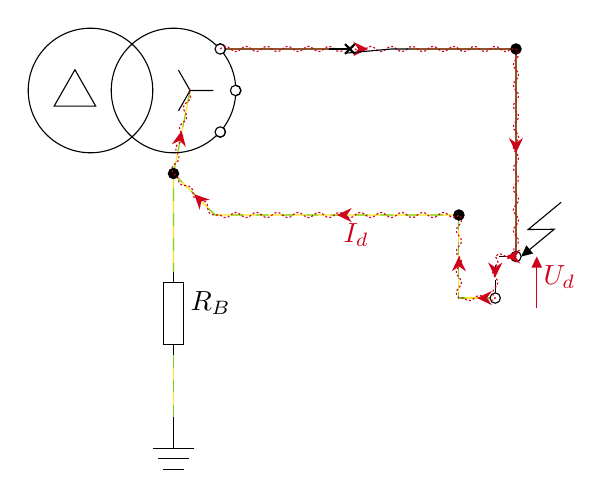
\begin{tikzpicture}[x=0.75pt,y=0.75pt,yscale=-1,xscale=1]
%uncomment if require: \path (0,251); %set diagram left start at 0, and has height of 251

%Straight Lines [id:da5104591094158853] 
\draw [color={rgb, 255:red, 248; green, 231; blue, 28 }  ,draw opacity=1 ]   (87.5,75) -- (107.5,95) -- (225,95) ;
%Straight Lines [id:da1966201814177917] 
\draw [color={rgb, 255:red, 126; green, 211; blue, 33 }  ,draw opacity=1 ] [dash pattern={on 4.5pt off 4.5pt}]  (87.5,75) -- (107.5,95) -- (225,95) ;
%Straight Lines [id:da3955266461919331] 
\draw [color={rgb, 255:red, 248; green, 231; blue, 28 }  ,draw opacity=1 ]   (87.5,162.5) -- (87.5,192.5) ;
%Straight Lines [id:da18836033833143995] 
\draw [color={rgb, 255:red, 248; green, 231; blue, 28 }  ,draw opacity=1 ]   (240,135) -- (225,135) -- (225,95) ;
%Straight Lines [id:da17249205616306007] 
\draw [color={rgb, 255:red, 139; green, 87; blue, 42 }  ,draw opacity=1 ]   (112.5,15) -- (162.5,15) ;
%Straight Lines [id:da11309897556582038] 
\draw [color={rgb, 255:red, 248; green, 231; blue, 28 }  ,draw opacity=1 ]   (95.5,35) -- (87.5,75) -- (87.5,122.5) ;
%Straight Lines [id:da4238452834369957] 
\draw [color={rgb, 255:red, 126; green, 211; blue, 33 }  ,draw opacity=1 ] [dash pattern={on 4.5pt off 4.5pt}]  (95.5,35) -- (87.5,75) -- (87.5,122.5) ;
%Straight Lines [id:da07337279365918903] 
\draw [color={rgb, 255:red, 139; green, 87; blue, 42 }  ,draw opacity=1 ]   (202.5,15) -- (252.5,15) ;
%Shape: Path Data [id:dp3633653751506416] 
\draw   (112.5,55) .. controls (112.5,56.38) and (111.38,57.5) .. (110,57.5) .. controls (109.29,57.5) and (108.65,57.2) .. (108.19,56.72) .. controls (102.81,61.85) and (95.52,65) .. (87.5,65) .. controls (70.93,65) and (57.5,51.57) .. (57.5,35) .. controls (57.5,18.43) and (70.93,5) .. (87.5,5) .. controls (95.52,5) and (102.81,8.15) .. (108.19,13.28) .. controls (108.65,12.8) and (109.29,12.5) .. (110,12.5) .. controls (111.38,12.5) and (112.5,13.62) .. (112.5,15) .. controls (112.5,15.82) and (112.11,16.54) .. (111.5,17) .. controls (114.8,21.39) and (116.92,26.71) .. (117.4,32.5) .. controls (117.43,32.5) and (117.47,32.5) .. (117.5,32.5) .. controls (118.88,32.5) and (120,33.62) .. (120,35) .. controls (120,36.38) and (118.88,37.5) .. (117.5,37.5) .. controls (117.47,37.5) and (117.43,37.5) .. (117.4,37.5) .. controls (116.92,43.29) and (114.8,48.61) .. (111.5,53) .. controls (112.11,53.46) and (112.5,54.18) .. (112.5,55) -- cycle ;
%Shape: Circle [id:dp8103241388904666] 
\draw   (17.5,35) .. controls (17.5,18.43) and (30.93,5) .. (47.5,5) .. controls (64.07,5) and (77.5,18.43) .. (77.5,35) .. controls (77.5,51.57) and (64.07,65) .. (47.5,65) .. controls (30.93,65) and (17.5,51.57) .. (17.5,35) -- cycle ;
%Shape: Triangle [id:dp1236855376591316] 
\draw   (40,25) -- (30,42.5) -- (50,42.5) -- cycle ;
%Shape: Star [id:dp7604780706337534] 
\draw   (106.75,35) -- (95.5,35) -- (89.88,44.81) -- (95.5,35) -- (89.88,25.19) -- (95.5,35) -- cycle ;
%Shape: Circle [id:dp9987526738268633] 
\draw   (107.5,15) .. controls (107.5,13.62) and (108.62,12.5) .. (110,12.5) .. controls (111.38,12.5) and (112.5,13.62) .. (112.5,15) .. controls (112.5,16.38) and (111.38,17.5) .. (110,17.5) .. controls (108.62,17.5) and (107.5,16.38) .. (107.5,15) -- cycle ;
%Shape: Circle [id:dp06603296247595714] 
\draw   (114.9,35) .. controls (114.9,33.62) and (116.02,32.5) .. (117.4,32.5) .. controls (118.78,32.5) and (119.9,33.62) .. (119.9,35) .. controls (119.9,36.38) and (118.78,37.5) .. (117.4,37.5) .. controls (116.02,37.5) and (114.9,36.38) .. (114.9,35) -- cycle ;
%Shape: Circle [id:dp9864995024391362] 
\draw   (107.5,55) .. controls (107.5,53.62) and (108.62,52.5) .. (110,52.5) .. controls (111.38,52.5) and (112.5,53.62) .. (112.5,55) .. controls (112.5,56.38) and (111.38,57.5) .. (110,57.5) .. controls (108.62,57.5) and (107.5,56.38) .. (107.5,55) -- cycle ;

%Straight Lines [id:da23296631733343887] 
\draw [color={rgb, 255:red, 139; green, 87; blue, 42 }  ,draw opacity=1 ]   (252.5,112.5) -- (252.5,17.5) ;
%Straight Lines [id:da9415376086031365] 
\draw [color={rgb, 255:red, 0; green, 0; blue, 0 }  ,draw opacity=1 ] [dash pattern={on 4.5pt off 4.5pt on 1pt off 4.5pt}]  (242.5,132.5) -- (242.5,115) -- (252.5,115) ;
%Straight Lines [id:da04537703273022686] 
\draw [color={rgb, 255:red, 126; green, 211; blue, 33 }  ,draw opacity=1 ] [dash pattern={on 4.5pt off 4.5pt}]  (240,135) -- (225,135) -- (225,95) ;
%Straight Lines [id:da014129266039552002] 
\draw    (87.5,192.5) -- (87.5,207.5) ;
%Straight Lines [id:da0064749529617041945] 
\draw    (77.5,207.5) -- (97.5,207.5) ;
%Straight Lines [id:da15495544426671526] 
\draw    (80,212.5) -- (95,212.5) ;
%Straight Lines [id:da9920646299152576] 
\draw    (82.5,217.5) -- (92.5,217.5) ;

%Straight Lines [id:da3741789060346865] 
\draw [color={rgb, 255:red, 126; green, 211; blue, 33 }  ,draw opacity=1 ] [dash pattern={on 4.5pt off 4.5pt}]  (87.5,162.5) -- (87.5,192.5) ;
%Straight Lines [id:da7734223518041439] 
\draw    (87.5,157.5) -- (87.5,162.5) ;
%Shape: Rectangle [id:dp997793865821069] 
\draw   (92.5,127.5) -- (92.5,157.5) -- (82.5,157.5) -- (82.5,127.5) -- cycle ;
%Straight Lines [id:da3149495431277475] 
\draw    (87.5,122.5) -- (87.5,127.5) ;

%Shape: Circle [id:dp16804091145958433] 
\draw  [fill={rgb, 255:red, 0; green, 0; blue, 0 }  ,fill opacity=1 ] (250,15) .. controls (250,13.62) and (251.12,12.5) .. (252.5,12.5) .. controls (253.88,12.5) and (255,13.62) .. (255,15) .. controls (255,16.38) and (253.88,17.5) .. (252.5,17.5) .. controls (251.12,17.5) and (250,16.38) .. (250,15) -- cycle ;
%Shape: Circle [id:dp448433802683451] 
\draw  [fill={rgb, 255:red, 255; green, 255; blue, 255 }  ,fill opacity=1 ] (240,135) .. controls (240,133.62) and (241.12,132.5) .. (242.5,132.5) .. controls (243.88,132.5) and (245,133.62) .. (245,135) .. controls (245,136.38) and (243.88,137.5) .. (242.5,137.5) .. controls (241.12,137.5) and (240,136.38) .. (240,135) -- cycle ;
%Shape: Circle [id:dp9631904407792523] 
\draw  [fill={rgb, 255:red, 255; green, 255; blue, 255 }  ,fill opacity=1 ] (250,115) .. controls (250,113.62) and (251.12,112.5) .. (252.5,112.5) .. controls (253.88,112.5) and (255,113.62) .. (255,115) .. controls (255,116.38) and (253.88,117.5) .. (252.5,117.5) .. controls (251.12,117.5) and (250,116.38) .. (250,115) -- cycle ;
%Shape: Circle [id:dp727181862391113] 
\draw  [fill={rgb, 255:red, 0; green, 0; blue, 0 }  ,fill opacity=1 ] (85,75) .. controls (85,73.62) and (86.12,72.5) .. (87.5,72.5) .. controls (88.88,72.5) and (90,73.62) .. (90,75) .. controls (90,76.38) and (88.88,77.5) .. (87.5,77.5) .. controls (86.12,77.5) and (85,76.38) .. (85,75) -- cycle ;
%Shape: Circle [id:dp14350658403367889] 
\draw  [fill={rgb, 255:red, 0; green, 0; blue, 0 }  ,fill opacity=1 ] (222.5,95) .. controls (222.5,93.62) and (223.62,92.5) .. (225,92.5) .. controls (226.38,92.5) and (227.5,93.62) .. (227.5,95) .. controls (227.5,96.38) and (226.38,97.5) .. (225,97.5) .. controls (223.62,97.5) and (222.5,96.38) .. (222.5,95) -- cycle ;
%Straight Lines [id:da09996473378362858] 
\draw [color={rgb, 255:red, 208; green, 2; blue, 27 }  ,draw opacity=1 ] [dash pattern={on 0.75pt off 0.75pt}]  (110,15) .. controls (111.67,13.33) and (113.33,13.33) .. (115,15) .. controls (116.67,16.67) and (118.33,16.67) .. (120,15) .. controls (121.67,13.33) and (123.33,13.33) .. (125,15) .. controls (126.67,16.67) and (128.33,16.67) .. (130,15) .. controls (131.67,13.33) and (133.33,13.33) .. (135,15) .. controls (136.67,16.67) and (138.33,16.67) .. (140,15) .. controls (141.67,13.33) and (143.33,13.33) .. (145,15) .. controls (146.67,16.67) and (148.33,16.67) .. (150,15) .. controls (151.67,13.33) and (153.33,13.33) .. (155,15) .. controls (156.67,16.67) and (158.33,16.67) .. (160,15) .. controls (161.67,13.33) and (163.33,13.33) .. (165,15) .. controls (166.67,16.67) and (168.33,16.67) .. (170,15) .. controls (171.67,13.33) and (173.33,13.33) .. (175,15) .. controls (176.67,16.67) and (178.33,16.67) .. (180,15) .. controls (181.67,13.33) and (183.33,13.33) .. (185,15) .. controls (186.67,16.67) and (188.33,16.67) .. (190,15) .. controls (191.67,13.33) and (193.33,13.33) .. (195,15) .. controls (196.67,16.67) and (198.33,16.67) .. (200,15) .. controls (201.67,13.33) and (203.33,13.33) .. (205,15) .. controls (206.67,16.67) and (208.33,16.67) .. (210,15) .. controls (211.67,13.33) and (213.33,13.33) .. (215,15) .. controls (216.67,16.67) and (218.33,16.67) .. (220,15) .. controls (221.67,13.33) and (223.33,13.33) .. (225,15) .. controls (226.67,16.67) and (228.33,16.67) .. (230,15) .. controls (231.67,13.33) and (233.33,13.33) .. (235,15) .. controls (236.67,16.67) and (238.33,16.67) .. (240,15) .. controls (241.67,13.33) and (243.33,13.33) .. (245,15) .. controls (246.67,16.67) and (248.33,16.67) .. (250,15) -- (252.5,15) -- (252.5,15) .. controls (254.17,16.67) and (254.17,18.33) .. (252.5,20) .. controls (250.83,21.67) and (250.83,23.33) .. (252.5,25) .. controls (254.17,26.67) and (254.17,28.33) .. (252.5,30) .. controls (250.83,31.67) and (250.83,33.33) .. (252.5,35) .. controls (254.17,36.67) and (254.17,38.33) .. (252.5,40) .. controls (250.83,41.67) and (250.83,43.33) .. (252.5,45) .. controls (254.17,46.67) and (254.17,48.33) .. (252.5,50) .. controls (250.83,51.67) and (250.83,53.33) .. (252.5,55) .. controls (254.17,56.67) and (254.17,58.33) .. (252.5,60) .. controls (250.83,61.67) and (250.83,63.33) .. (252.5,65) .. controls (254.17,66.67) and (254.17,68.33) .. (252.5,70) .. controls (250.83,71.67) and (250.83,73.33) .. (252.5,75) .. controls (254.17,76.67) and (254.17,78.33) .. (252.5,80) .. controls (250.83,81.67) and (250.83,83.33) .. (252.5,85) .. controls (254.17,86.67) and (254.17,88.33) .. (252.5,90) .. controls (250.83,91.67) and (250.83,93.33) .. (252.5,95) .. controls (254.17,96.67) and (254.17,98.33) .. (252.5,100) .. controls (250.83,101.67) and (250.83,103.33) .. (252.5,105) .. controls (254.17,106.67) and (254.17,108.33) .. (252.5,110) .. controls (250.83,111.67) and (250.83,113.33) .. (252.5,115) -- (252.5,115) .. controls (250.83,116.67) and (249.17,116.67) .. (247.5,115) .. controls (245.83,113.33) and (244.17,113.33) .. (242.5,115) -- (242.5,115) .. controls (244.17,116.67) and (244.17,118.33) .. (242.5,120) .. controls (240.83,121.67) and (240.83,123.33) .. (242.5,125) .. controls (244.17,126.67) and (244.17,128.33) .. (242.5,130) .. controls (240.83,131.67) and (240.83,133.33) .. (242.5,135) -- (242.5,135) .. controls (240.83,136.67) and (239.17,136.67) .. (237.5,135) .. controls (235.83,133.33) and (234.17,133.33) .. (232.5,135) .. controls (230.83,136.67) and (229.17,136.67) .. (227.5,135) -- (225,135) -- (225,135) .. controls (223.33,133.33) and (223.33,131.67) .. (225,130) .. controls (226.67,128.33) and (226.67,126.67) .. (225,125) .. controls (223.33,123.33) and (223.33,121.67) .. (225,120) .. controls (226.67,118.33) and (226.67,116.67) .. (225,115) .. controls (223.33,113.33) and (223.33,111.67) .. (225,110) .. controls (226.67,108.33) and (226.67,106.67) .. (225,105) .. controls (223.33,103.33) and (223.33,101.67) .. (225,100) .. controls (226.67,98.33) and (226.67,96.67) .. (225,95) -- (225,95) .. controls (223.33,96.67) and (221.67,96.67) .. (220,95) .. controls (218.33,93.33) and (216.67,93.33) .. (215,95) .. controls (213.33,96.67) and (211.67,96.67) .. (210,95) .. controls (208.33,93.33) and (206.67,93.33) .. (205,95) .. controls (203.33,96.67) and (201.67,96.67) .. (200,95) .. controls (198.33,93.33) and (196.67,93.33) .. (195,95) .. controls (193.33,96.67) and (191.67,96.67) .. (190,95) .. controls (188.33,93.33) and (186.67,93.33) .. (185,95) .. controls (183.33,96.67) and (181.67,96.67) .. (180,95) .. controls (178.33,93.33) and (176.67,93.33) .. (175,95) .. controls (173.33,96.67) and (171.67,96.67) .. (170,95) .. controls (168.33,93.33) and (166.67,93.33) .. (165,95) .. controls (163.33,96.67) and (161.67,96.67) .. (160,95) .. controls (158.33,93.33) and (156.67,93.33) .. (155,95) .. controls (153.33,96.67) and (151.67,96.67) .. (150,95) .. controls (148.33,93.33) and (146.67,93.33) .. (145,95) .. controls (143.33,96.67) and (141.67,96.67) .. (140,95) .. controls (138.33,93.33) and (136.67,93.33) .. (135,95) .. controls (133.33,96.67) and (131.67,96.67) .. (130,95) .. controls (128.33,93.33) and (126.67,93.33) .. (125,95) .. controls (123.33,96.67) and (121.67,96.67) .. (120,95) .. controls (118.33,93.33) and (116.67,93.33) .. (115,95) .. controls (113.33,96.67) and (111.67,96.67) .. (110,95) -- (107.5,95) -- (107.5,95) .. controls (105.14,95) and (103.96,93.82) .. (103.96,91.46) .. controls (103.96,89.11) and (102.78,87.93) .. (100.43,87.93) .. controls (98.07,87.93) and (96.89,86.75) .. (96.89,84.39) .. controls (96.89,82.04) and (95.71,80.86) .. (93.36,80.86) .. controls (91,80.86) and (89.82,79.68) .. (89.82,77.32) -- (87.5,75) -- (87.5,75) .. controls (86.17,73.05) and (86.48,71.42) .. (88.43,70.09) .. controls (90.38,68.76) and (90.69,67.12) .. (89.36,65.17) .. controls (88.03,63.22) and (88.34,61.59) .. (90.29,60.26) .. controls (92.24,58.93) and (92.54,57.3) .. (91.21,55.35) .. controls (89.88,53.4) and (90.19,51.77) .. (92.14,50.44) .. controls (94.09,49.11) and (94.4,47.47) .. (93.07,45.52) .. controls (91.74,43.57) and (92.05,41.94) .. (94,40.61) .. controls (95.95,39.28) and (96.26,37.65) .. (94.93,35.7) -- (95.25,34) -- (95.25,34) ;
\draw [shift={(181.25,15)}, rotate = 180] [fill={rgb, 255:red, 208; green, 2; blue, 27 }  ,fill opacity=1 ][line width=0.08]  [draw opacity=0] (7.14,-3.43) -- (0,0) -- (7.14,3.43) -- (4.74,0) -- cycle    ;
\draw [shift={(252.5,65)}, rotate = 270] [fill={rgb, 255:red, 208; green, 2; blue, 27 }  ,fill opacity=1 ][line width=0.08]  [draw opacity=0] (7.14,-3.43) -- (0,0) -- (7.14,3.43) -- (4.74,0) -- cycle    ;
\draw [shift={(247.5,115)}, rotate = 360] [fill={rgb, 255:red, 208; green, 2; blue, 27 }  ,fill opacity=1 ][line width=0.08]  [draw opacity=0] (7.14,-3.43) -- (0,0) -- (7.14,3.43) -- (4.74,0) -- cycle    ;
\draw [shift={(242.5,125)}, rotate = 270] [fill={rgb, 255:red, 208; green, 2; blue, 27 }  ,fill opacity=1 ][line width=0.08]  [draw opacity=0] (7.14,-3.43) -- (0,0) -- (7.14,3.43) -- (4.74,0) -- cycle    ;
\draw [shift={(233.75,135)}, rotate = 360] [fill={rgb, 255:red, 208; green, 2; blue, 27 }  ,fill opacity=1 ][line width=0.08]  [draw opacity=0] (7.14,-3.43) -- (0,0) -- (7.14,3.43) -- (4.74,0) -- cycle    ;
\draw [shift={(225,115)}, rotate = 450] [fill={rgb, 255:red, 208; green, 2; blue, 27 }  ,fill opacity=1 ][line width=0.08]  [draw opacity=0] (7.14,-3.43) -- (0,0) -- (7.14,3.43) -- (4.74,0) -- cycle    ;
\draw [shift={(166.25,95)}, rotate = 360] [fill={rgb, 255:red, 208; green, 2; blue, 27 }  ,fill opacity=1 ][line width=0.08]  [draw opacity=0] (7.14,-3.43) -- (0,0) -- (7.14,3.43) -- (4.74,0) -- cycle    ;
\draw [shift={(97.5,85)}, rotate = 405] [fill={rgb, 255:red, 208; green, 2; blue, 27 }  ,fill opacity=1 ][line width=0.08]  [draw opacity=0] (7.14,-3.43) -- (0,0) -- (7.14,3.43) -- (4.74,0) -- cycle    ;
\draw [shift={(91.38,54.5)}, rotate = 460.7] [fill={rgb, 255:red, 208; green, 2; blue, 27 }  ,fill opacity=1 ][line width=0.08]  [draw opacity=0] (7.14,-3.43) -- (0,0) -- (7.14,3.43) -- (4.74,0) -- cycle    ;
%Shape: Boxed Line [id:dp3673372749832414] 
\draw    (274.27,88.83) -- (258.39,101.97) -- (270.89,101.86) -- (257.31,113.09) ;
\draw [shift={(255,115)}, rotate = 320.40999999999997] [fill={rgb, 255:red, 0; green, 0; blue, 0 }  ][line width=0.08]  [draw opacity=0] (5.36,-2.57) -- (0,0) -- (5.36,2.57) -- cycle    ;
%Straight Lines [id:da5575509867036751] 
\draw    (170.5,17) -- (192.5,15) -- (202.5,15) ;
%Straight Lines [id:da508912305096757] 
\draw    (172.5,15) -- (162.5,15) ;
\draw [shift={(172.5,15)}, rotate = 225] [color={rgb, 255:red, 0; green, 0; blue, 0 }  ][line width=0.75]    (-3.35,0) -- (3.35,0)(0,3.35) -- (0,-3.35)   ;

%Straight Lines [id:da16958097231268054] 
\draw [color={rgb, 255:red, 208; green, 2; blue, 27 }  ,draw opacity=1 ]   (262.5,118) -- (262.5,140) ;
\draw [shift={(262.5,115)}, rotate = 90] [fill={rgb, 255:red, 208; green, 2; blue, 27 }  ,fill opacity=1 ][line width=0.08]  [draw opacity=0] (5.36,-2.57) -- (0,0) -- (5.36,2.57) -- cycle    ;

% Text Node
\draw (94.5,130.5) node [anchor=north west][inner sep=0.75pt]   [align=left] {$R_B$};
% Text Node
\draw (168.25,98) node [anchor=north west][inner sep=0.75pt]  [color={rgb, 255:red, 208; green, 2; blue, 27 }  ,opacity=1 ] [align=left] {$I_d$};
% Text Node
\draw (264.5,118) node [anchor=north west][inner sep=0.75pt]  [color={rgb, 255:red, 208; green, 2; blue, 27 }  ,opacity=1 ] [align=left] {$U_d$};


\end{tikzpicture}

\end{figure}

%\end{document}

